% ============================ 01 前向推理 ============================

\section{前向推理：候选轨迹的生成}

\begin{frame}[plain]
  \begin{center}
    \vspace{1.2cm}
    {\color{yopoblue}\Huge\bfseries 01}\\[0.5em]
    {\color{yopoblue}\LARGE 前向推理：候选轨迹的生成}\\[1.2em]
    \begin{minipage}{0.72\textwidth}
      \small\color{yopogray}
      候选轨迹由\textbf{固定锚点}、\textbf{网络预测的有界修正量}与\textbf{五次多项式解析解}共同构成。
      网络仅输出其中的修正量与终端导数，不直接输出曲线。
    \end{minipage}
  \end{center}
\end{frame}

% ---------------------------------------------------------------
\begin{frame}[shrink=12]{规划的多模态性与多候选结构}
  \noindent
  \begin{minipage}[t]{0.4\textwidth}\vspace{0pt}
      \scriptsize
      \begin{block}{问题}
        \begin{itemize}\tight
          \item 左绕、右绕都可行，都存在合理解；
          \item 单一回归头把它压成一个输出 $\Rightarrow$ \textbf{折中解}；
          \item 多假设 + winner-takes-all $\Rightarrow$ \textbf{模式坍缩}。
        \end{itemize}
      \end{block}
  \end{minipage}\hfill
  \begin{minipage}[t]{0.57\textwidth}\vspace{0pt}
      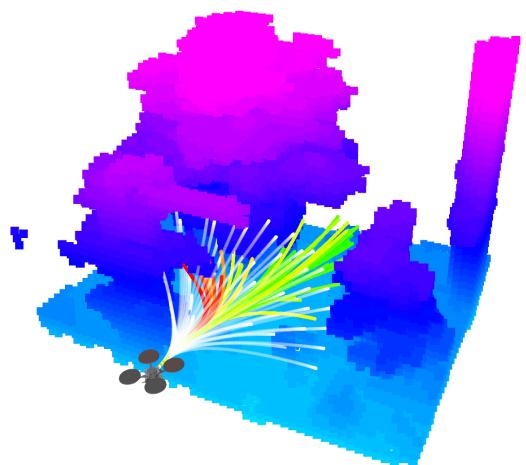
\includegraphics[width=0.74\linewidth]{figures/01_anchor_exploration.jpg}
      \begin{center}\scriptsize\color{yopogray}
      原文 Fig.~1：白线为运动基元锚点，\\
      彩色曲线为按评分着色的预测结果
      \end{center}
  \end{minipage}
  \begin{paperfinding}[原文的解法]
    \scriptsize
    借鉴 YOLO 的“\textbf{锚框 + 偏移}”结构：
    在相机视场内均匀铺开一组运动基元作为\textbf{锚点}，
    让每个输出位置只负责自己那片局部解空间，
    再预测该候选的\textbf{改进量}与\textbf{质量}。
  \end{paperfinding}
\end{frame}

% ---------------------------------------------------------------
\begin{frame}{运动基元锚点的球坐标定义}
  \small
  \begin{columns}[t]
    \begin{column}{0.54\textwidth}
      以本轮规划开始时的机体坐标系表示，第 $(i,j)$ 个锚点为（原文式 (3)）：
      \[
        \mathbf p_{ij}=\bigl(r\cos\theta_j\cos\varphi_i,\;
        r\cos\theta_j\sin\varphi_i,\; r\sin\theta_j\bigr)
      \]
      \begin{itemize}\tight
        \item $\varphi_i$：水平方位角，共 $M_\varphi$ 个；
        \item $\theta_j$：竖直方向角，共 $M_\theta$ 个；
        \item $r$：基准规划半径（对应规划时域）。
      \end{itemize}
      \begin{reading}[基元库的表达空间]
        \scriptsize
        原文明确：基元库定义在 \textbf{state lattice space} 而不是多项式系数空间。
        这样表达是“\textbf{空间分离}”的——每个候选占一块位置，
        才能与卷积特征图的每个格子一一对上。
      \end{reading}
    \end{column}
    \begin{column}{0.42\textwidth}
      \begin{block}{论文实验配置}
        \scriptsize
        \begin{tabular}{@{}ll@{}}
          \toprule
          水平数 $M_\varphi$ & 5 \\
          竖直数 $M_\theta$ & 3 \\
          候选总数 & $\mathbf{15}$ \\
          相机视场（配置） & $90^\circ\times60^\circ$ \\
          图像分辨率 & $160\times96$ \\
          基准半径 $r$（配置） & 4\,m \\
          \bottomrule
        \end{tabular}
      \end{block}
      \begin{reading}
        \scriptsize
        “15 个”是\textbf{实验配置}，不是方法要求的固定常数。
        候选数由图像分辨率与下采样倍数共同决定。
      \end{reading}
    \end{column}
  \end{columns}
\end{frame}

% ---------------------------------------------------------------
\begin{frame}[shrink=12]{锚点的具体取值}
  \noindent
  \begin{minipage}[t]{0.55\textwidth}\vspace{0pt}
      \begin{block}{均匀采样 $\Rightarrow$ 具体角度}
        \scriptsize
        \textbf{水平}：步长 $90^\circ/5=18^\circ$，取 5 个格子中心
        \[
          \varphi_i \in \{-36^\circ,-18^\circ,\;0^\circ,+18^\circ,+36^\circ\}
        \]
        \textbf{竖直}：步长 $60^\circ/3=20^\circ$，取 3 个格子中心
        $\theta_j \in \{-20^\circ,\;0^\circ,+20^\circ\}$。\\
        每个锚点半径 $r=4$\,m，共 $5\times3=15$ 个锚点。
      \end{block}
  \end{minipage}\hfill
  \begin{minipage}[t]{0.41\textwidth}\vspace{0pt}
      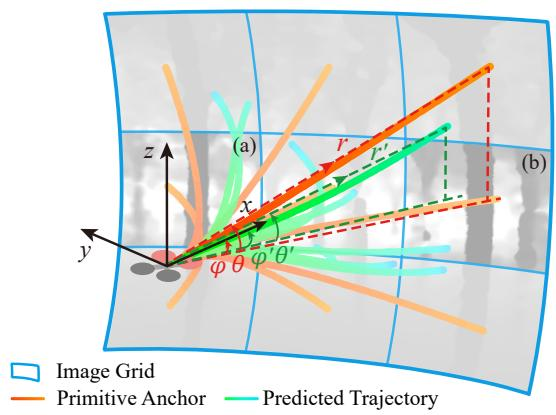
\includegraphics[width=0.9\linewidth]{figures/04_primitive_definition.jpg}
      \begin{center}\scriptsize\color{yopogray}
      原文 Fig.~4：深度图被划分为 $M_\varphi\times M_\theta$ 个格子，
      每个格子对应视锥内的一个基元
      \end{center}
  \end{minipage}
  \begin{reading}[数值来源]
    \scriptsize
    $\pm36^\circ/\pm20^\circ$ 由原文“在传感器可见范围内均匀采样”
    $+$ $5\times3$ 网格 $+$ 配置视场 $90^\circ\times60^\circ$ 推出；
    视场角与半径取自作者开源配置，论文正文只给出相机型号与图像分辨率。
  \end{reading}
\end{frame}

% ---------------------------------------------------------------
\begin{frame}{网络输出：锚点的有界修正量}
  \small
  \begin{columns}[t]
    \begin{column}{0.52\textwidth}
      对每个锚点，网络输出 3 个偏移量，用 $\tanh$ 夹在有界范围内（原文式 (8)）：
      \[
        \begin{aligned}
          \Delta\theta &= \tanh(y_\theta)\,d_\theta\\
          \Delta\varphi &= \tanh(y_\varphi)\,d_\varphi\\
          \Delta r &= \tanh(y_r)\,d_r
        \end{aligned}
      \]
      修正后的终端位置（原文式 (4)）：
      \[
        r'=r+\Delta r,\quad \varphi'=\varphi_i+\Delta\varphi,\quad \theta'=\theta_j+\Delta\theta
      \]
      再代回同一套球坐标变换得到 $\mathbf p_T$。
    \end{column}
    \begin{column}{0.44\textwidth}
      \begin{block}{偏移窗口 vs 格子大小}
        \footnotesize
        \begin{tabular}{@{}lcc@{}}
          \toprule
          方向 & 格子间距 & 偏移窗口（配置） \\
          \midrule
          水平 & $18^\circ$ & $\pm15^\circ$（共 $30^\circ$）\\
          竖直 & $20^\circ$ & $\pm15^\circ$（共 $30^\circ$）\\
          半径 & $r=4$\,m & $\pm4$\,m $\Rightarrow r'\in[0,8]$ \\
          \bottomrule
        \end{tabular}
      \end{block}
      \begin{paperfinding}[关键设计：窗口略大于格子]
        \footnotesize
        原文：“局部解空间先验\textbf{略大于}格子的视场”，
        因此相邻候选的区域可以\textbf{重叠}——
        这既保证候选互相分散（多模态），又不让它们完全无法协调。
      \end{paperfinding}
    \end{column}
  \end{columns}
\end{frame}

% ---------------------------------------------------------------
\begin{frame}{锚点可达域：球面格点与单个扇区}
  \begin{center}
    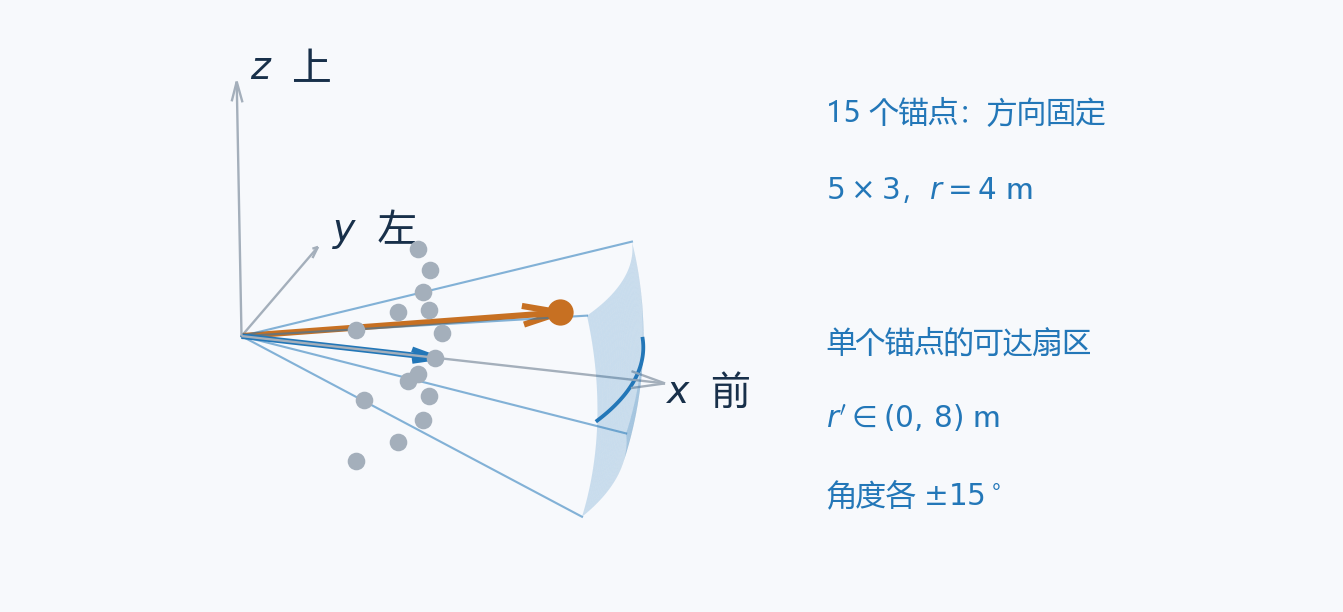
\includegraphics[width=\linewidth]{figures/24a_primitive_sector.png}
  \end{center}
\end{frame}

% ---------------------------------------------------------------
\begin{frame}{水平剖面：角度窗口与半径修正}
  \begin{center}
    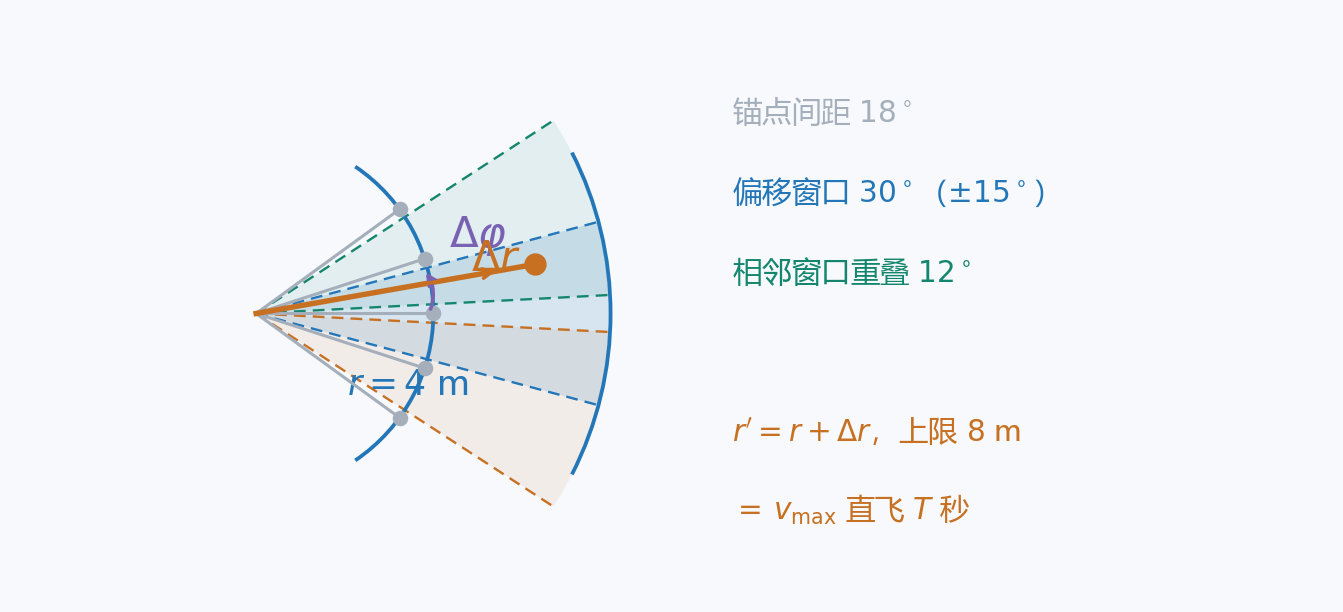
\includegraphics[width=\linewidth]{figures/24b_primitive_section.png}
  \end{center}
\end{frame}

% ---------------------------------------------------------------
\begin{frame}{基元坐标系与机体坐标系的变换关系}
  \begin{center}
    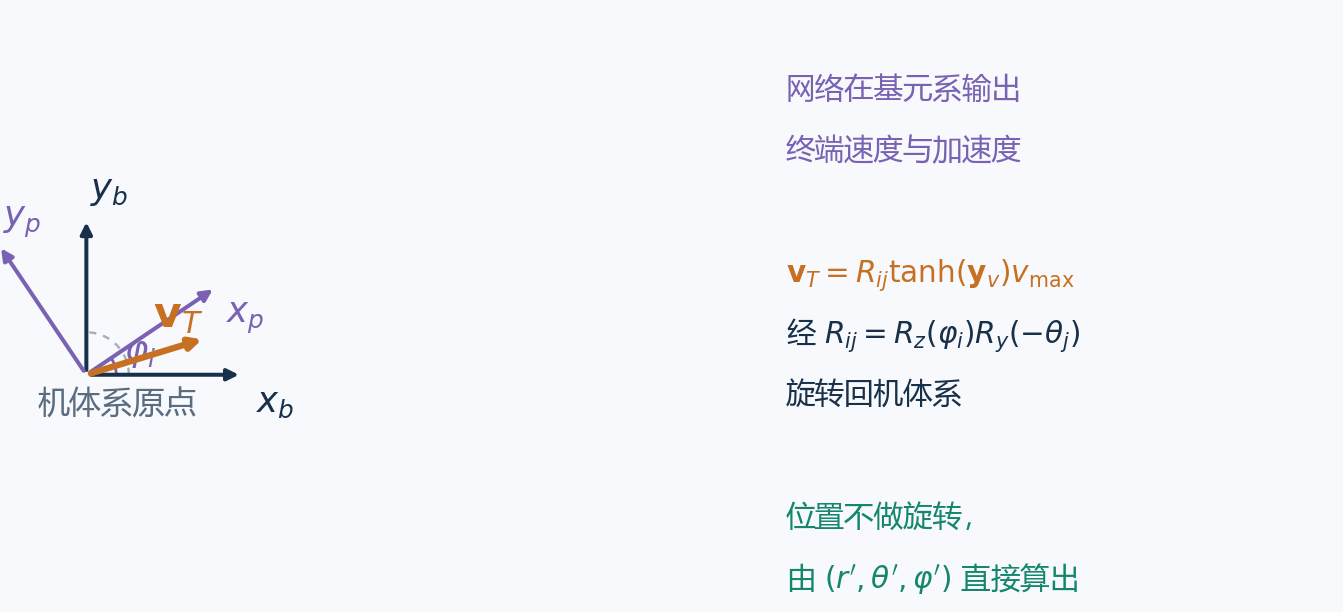
\includegraphics[width=\linewidth]{figures/24c_frame_rotation.png}
  \end{center}
\end{frame}

% ---------------------------------------------------------------
\begin{frame}[shrink=6]{终端速度与加速度的预测}
  \small
  \begin{columns}[t]
    \begin{column}{0.5\textwidth}
      \small
      终端导数同样经 $\tanh$ 限幅，再从基元系转回机体系（原文式 (9)）：
      \[
        \begin{aligned}
          \mathbf v_T &= R_{ij}\,\tanh(\mathbf y_v)\,v_{\max}\\
          \mathbf a_T &= R_{ij}\,\tanh(\mathbf y_a)\,a_{\max}
        \end{aligned}
      \]
      \begin{itemize}\tight
        \item $R_{ij}$：基元系 $\to$ 机体系的旋转（式 (6)）；
        \item 限幅的目的：\textbf{动力学可行}——
              终端速度/加速度不会超出训练分布。
      \end{itemize}
    \end{column}
    \begin{column}{0.46\textwidth}
      \begin{reading}[终端状态的信息量]
        \scriptsize
        终点位置相同、终端速度/加速度不同，整条曲线的形状仍然不同。
        所以网络输出的 9 个数比“一个目标点”信息量大得多，
        它同时表达了\textbf{靠近的方式}。
      \end{reading}
      \begin{reading}[限幅的作用范围]
        \scriptsize
        对\textbf{输出分量}限幅，不能直接解释为对整条轨迹的速度模长、
        推力或角速度的严格保证。
      \end{reading}
    \end{column}
  \end{columns}
\end{frame}

% ---------------------------------------------------------------
\begin{frame}{网络结构：ResNet-18 主干 + 共享 $1\times1$ 卷积头}
  \small
  \begin{columns}[t]
    \begin{column}{0.55\textwidth}
      \begin{block}{张量形状流（批次 $B$）}
        \scriptsize
        \begin{tabular}{@{}lll@{}}
          \toprule
          数据 & 形状 & 说明 \\
          \midrule
          深度图 & $B{\times}1{\times}96{\times}160$ & 单通道深度 \\
          图像特征 & $B{\times}64{\times}3{\times}5$ & ResNet-18，32 倍下采样 \\
          状态张量 & $B{\times}9{\times}3{\times}5$ & 每个基元一份坐标变换 \\
          头输入 & $B{\times}73{\times}3{\times}5$ & $64+9$ 通道拼接 \\
          原始输出 & $B{\times}10{\times}3{\times}5$ & 每个格子 10 个数 \\
          可重排为 & $B{\times}15{\times}10$ & 15 组“9 参数 + 1 评分” \\
          \bottomrule
        \end{tabular}
      \end{block}
    \end{column}
    \begin{column}{0.41\textwidth}
      \begin{itemize}\tight
        \item 主干是\textbf{改过的 ResNet-18}：单通道输入、
              去掉平均池化、$1\times1$ 卷积输出 64 通道特征图；
        \item 预测头是三层 $1\times1$ 卷积（256–256–10），\textbf{权重共享}；
        \item 状态分支是一个\textbf{空的 Sequential}——
              状态几乎只做几何处理，不经过额外网络层。
      \end{itemize}
      \begin{reading}
        \scriptsize
        15 个候选是\textbf{一次张量计算}并行产出的：
        共享骨干张量上的不同空间位置，
        不是 15 个线程或 15 个独立网络。
      \end{reading}
    \end{column}
  \end{columns}
\end{frame}

% ---------------------------------------------------------------
\begin{frame}{特征图网格与运动基元的空间对应}
  \small
  \begin{columns}[t]
    \begin{column}{0.52\textwidth}
      \begin{block}{几何上的对应关系}
        \footnotesize
        下采样 32 倍：$96\times160 \longrightarrow 3\times5$。
        特征图的 \textbf{3 行 = 竖直 3 个基元}，
        \textbf{5 列 = 水平 5 个基元}——格子与锚点一一对应。
      \end{block}
      \begin{reading}[必须澄清的一点]
        \small
        对应关系是\textbf{位置级}的，不是“信息隔离”的：
        卷积感受野覆盖整张图，
        \textbf{每个格子看到的是全局上下文的特征}，
        而不是自己视锥那一小块。
      \end{reading}
    \end{column}
    \begin{column}{0.44\textwidth}
      \begin{block}{与图像格子编号的错位}
        \footnotesize
        格子的行优先展开顺序与基元的极坐标索引顺序\textbf{相反}
        （图像从左到右、从下到上，而基元按另一顺序编号），
        实现时需要一次索引翻转：
        \[
          \text{grid} \;\leftrightarrow\; \text{lattice}=14-\text{grid}
        \]
        这只影响实现，不改变物理含义。
      \end{block}
    \end{column}
  \end{columns}
\end{frame}

% ---------------------------------------------------------------
\begin{frame}{基元坐标系：规划问题的非平移不变性}
  \small
  \begin{columns}[t]
    \begin{column}{0.5\textwidth}
      原文式 (6)：机体 $\to$ 基元的旋转
      \[
        R_{ij}=R_z(\varphi_i)R_y(-\theta_j)
      \]
      原文式 (7)：输入状态变换到基元系
      \[
        \mathbf x'_{ij}=R_{ij}^{-1}\mathbf x
      \]
      $R_{ij}$ 的直观含义：
      “把机体系下的状态，表达成\textbf{相对于这个候选方向}的量”。
    \end{column}
    \begin{column}{0.46\textwidth}
      \begin{paperfinding}[矛盾在哪里]
        \small
        图 4 中，左侧格子 (a) 需要“向右”的偏移，
        右侧格子 (b) 需要“向左”的偏移——
        \textbf{同样的特征，期望的输出相反}。
        共享权重的卷积头无法同时满足，
        除非输入被表达成“相对量”。
      \end{paperfinding}
      \begin{reading}
        \scriptsize
        这正是 $1\times1$ 卷积共享权重能成立的前提：
        不是让网络学会 15 套规则，而是把 15 个问题\textbf{归一化成同一个问题}。
      \end{reading}
    \end{column}
  \end{columns}
\end{frame}

% ---------------------------------------------------------------
\begin{frame}{状态输入的构造与坐标变换}
  \small
  \begin{columns}[t]
    \begin{column}{0.54\textwidth}
      \begin{block}{输入状态的构造}
        \footnotesize
        \begin{itemize}\tight
          \item 机体系 9 维状态：速度(3) + 加速度(3) + 目标单位方向(3)；
          \item 归一化：$\mathbf v/v_{\max}$、$\mathbf a/a_{\max}$、
                目标方向单位化并设下限（避免除零）；
          \item 对每个基元旋转一次：
                $\mathbf x'_{ij}=[\;R_{ij}^{-1}\mathbf v,\;R_{ij}^{-1}\mathbf a,\;R_{ij}^{-1}\hat{\mathbf g}\;]$
          \item 得到 $B\times9\times3\times5$，与图像特征\textbf{按通道拼接}。
        \end{itemize}
      \end{block}
    \end{column}
    \begin{column}{0.42\textwidth}
      \begin{reading}[实现上的常见错误]
        \small
        9 维状态是\textbf{三个 3 维向量}，需分别旋转；
        不能用一个 $3\times3$ 矩阵去乘 $9\times1$ 的向量。
        等价写法是块对角矩阵
        $\operatorname{diag}(R^{-1},R^{-1},R^{-1})$。
      \end{reading}
      \begin{reading}[方向约定]
        \scriptsize
        按原文式 (7)(9)：机体系向量转到基元系用 $R_{ij}^{-1}$，
        基元系终端导数转回机体系用 $R_{ij}$。
        实现时应依此核对方向，避免仅凭矩阵名称判断。
      \end{reading}
    \end{column}
  \end{columns}
\end{frame}

% ---------------------------------------------------------------
\begin{frame}{候选输出参数：每组 10 个分量}
  \small
  \begin{columns}[t]
    \begin{column}{0.5\textwidth}
      第 $i$ 个候选的原始输出向量：
      \[
        \mathbf y_i=\bigl[y_\theta,\;y_\varphi,\;y_r,\;
        \mathbf y_v^{\mathsf T},\;\mathbf y_a^{\mathsf T},\;\hat s_i\bigr]^{\mathsf T}
      \]
      前 9 个经偏移、限幅与旋转，得到有物理意义的终端状态：
      \[
        \mathbf q_i=\bigl[\mathbf p_{T,i}^{\mathsf T},\;
        \mathbf v_{T,i}^{\mathsf T},\;\mathbf a_{T,i}^{\mathsf T}\bigr]^{\mathsf T}\in\mathbb R^9
      \]
      第 10 个 $\hat s_i$ 是\textbf{该候选的代价估计}（评分）。
    \end{column}
    \begin{column}{0.46\textwidth}
      \begin{block}{10 个输出的分工}
        \footnotesize
        \begin{tabular}{@{}cll@{}}
          \toprule
          序号 & 含义 & 解码 \\
          \midrule
          1 & 方位角偏移 & $\tanh\cdot15^\circ$ \\
          2 & 俯仰角偏移 & $\tanh\cdot15^\circ$ \\
          3 & 半径偏移 & $\tanh\cdot r$ \\
          4--6 & 终端速度 & $R\tanh\cdot v_{\max}$ \\
          7--9 & 终端加速度 & $R\tanh\cdot a_{\max}$ \\
          10 & 评分 & 单调激活 \\
          \bottomrule
        \end{tabular}
      \end{block}
      \begin{reading}
        \scriptsize
        评分与轨迹参数从\textbf{同一组共享特征}中同时产生；
        评分不是另一个“接收完整曲线、在线查地图”的独立评价网络。
      \end{reading}
    \end{column}
  \end{columns}
\end{frame}

% ---------------------------------------------------------------
\begin{frame}{从终端状态到连续曲线：五次多项式边界值问题}
  \small
  \begin{columns}[t]
    \begin{column}{0.52\textwidth}
      对任一轴 $\mu\in\{x,y,z\}$（原文式 (1)(2)(5)）：
      \[
        p_\mu(t)=c_0+c_1t+c_2t^2+c_3t^3+c_4t^4+c_5t^5
      \]
      把\textbf{当前状态}与\textbf{终端状态}组成边界向量 $\mathbf d$，
      用常数矩阵映射到系数（原文式 (5)）：
      \[
        \mathbf c_\mu = M(T)^{-1}\mathbf d_\mu
      \]
      \[
        M(T)=
        \begin{bmatrix}
          1&0&0&0&0&0\\
          0&1&0&0&0&0\\
          0&0&2&0&0&0\\
          1&T&T^2&T^3&T^4&T^5\\
          0&1&2T&3T^2&4T^3&5T^4\\
          0&0&2&6T&12T^2&20T^3
        \end{bmatrix}
      \]
    \end{column}
    \begin{column}{0.44\textwidth}
      \begin{block}{六个边界条件}
        \footnotesize
        起点：位置 $\mathbf p_0$、速度 $\mathbf v_0$、加速度 $\mathbf a_0$\\
        终点：位置 $\mathbf p_T$、速度 $\mathbf v_T$、加速度 $\mathbf a_T$
      \end{block}
      \begin{reading}[三个轴各解一次]
        \small
        三个轴分别求解，共 18 个系数。
        $T>0$ 时矩阵可逆、解唯一，且固定 $T$ 后可\textbf{预先算好} $M(T)^{-1}$——
        在线求解只是几次矩阵乘。
      \end{reading}
      \begin{reading}[不提供什么保证]
        \scriptsize
        单段多项式保证连续可导并精确满足边界条件，
        \textbf{不自动保证无碰撞}或满足全部动力学硬约束。
      \end{reading}
    \end{column}
  \end{columns}
\end{frame}

% ---------------------------------------------------------------
\begin{frame}{在线推理流程}
  \begin{columns}[c]
    \begin{column}{0.55\textwidth}
      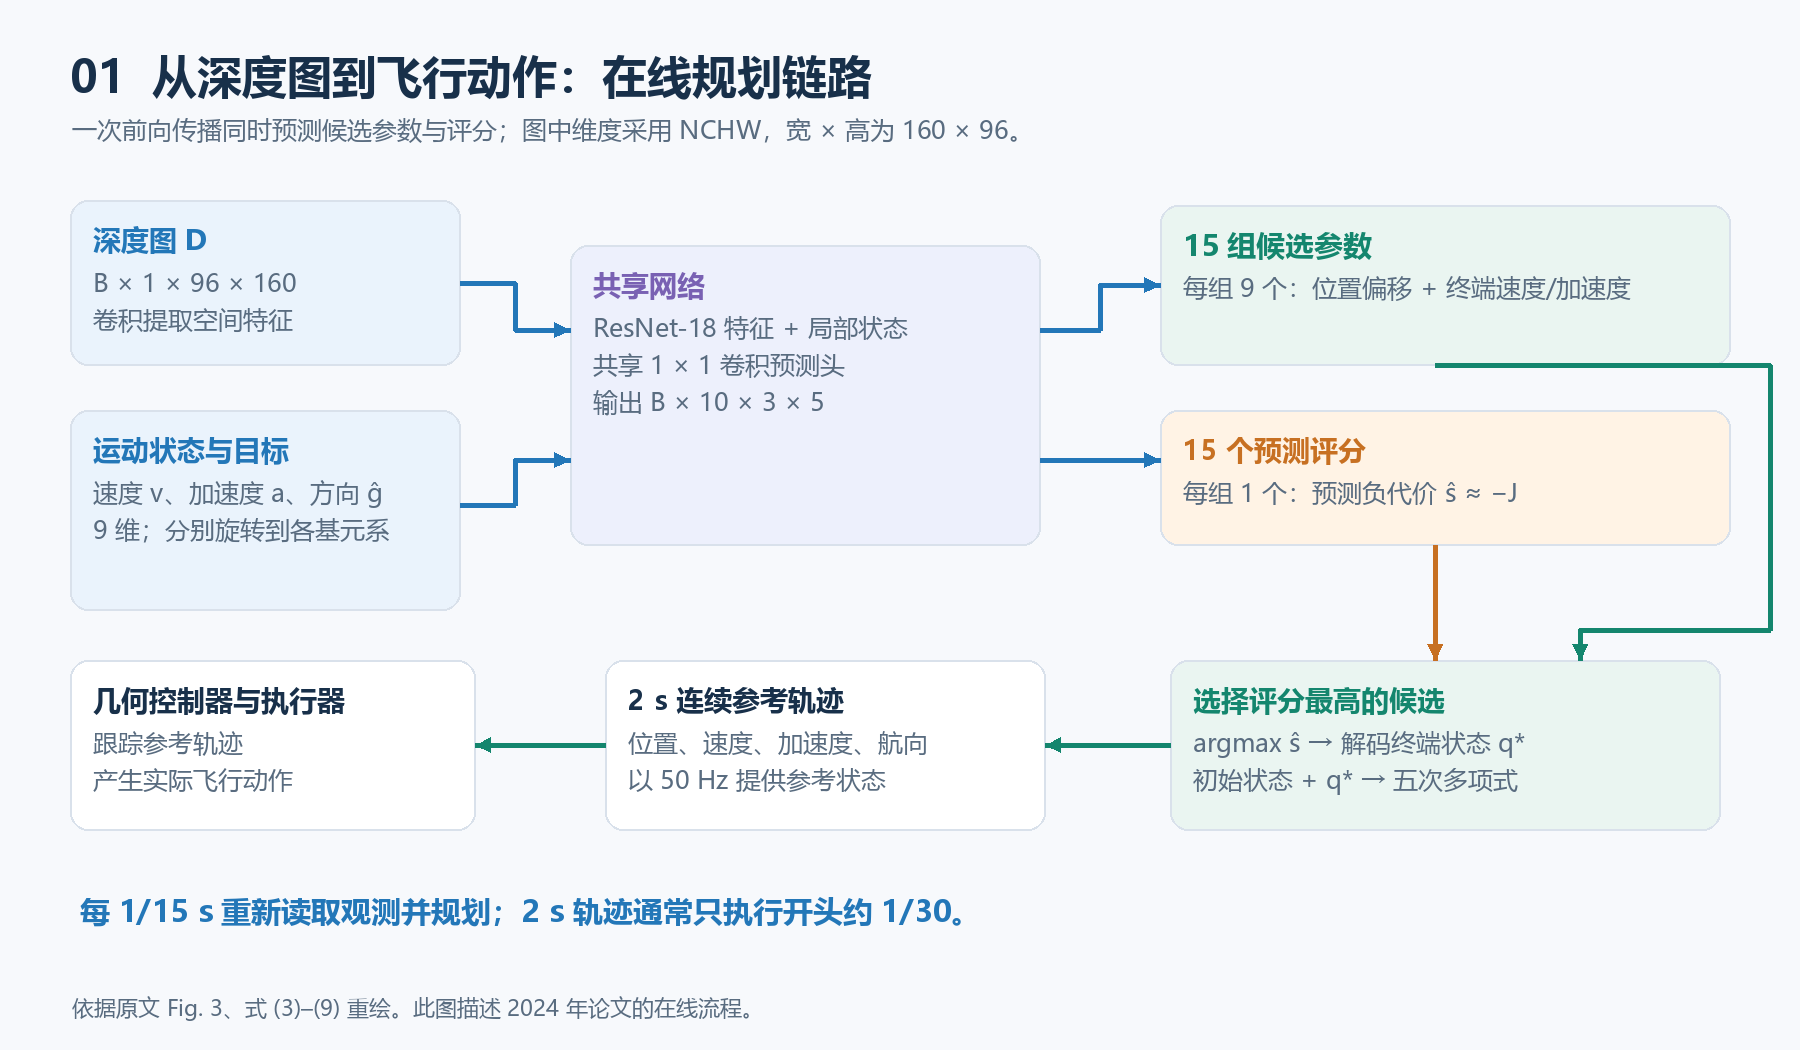
\includegraphics[width=\linewidth]{figures/20_note_online_pipeline.png}
    \end{column}
    \begin{column}{0.43\textwidth}
      \small
      \footnotesize
      \begin{enumerate}\tight
        \item 取深度图 + 当前速度、加速度、目标方向；
        \item 提特征、把状态变换到各基元系并拼接；
        \item 共享头同时输出 \textbf{15 组轨迹参数 + 15 个评分}；
        \item 选\textbf{评分最好}的候选，解码其终端状态；
        \item 代入边界值问题，求出五次多项式；
        \item 输出参考位置、速度、加速度、航向给控制器。
      \end{enumerate}
      \begin{paperfinding}[算力上的关键]
        \scriptsize
        在线\textbf{只对选中的那条轨迹求解多项式}；
        另外 14 条只是网络输出，不进入求解、不查地图。
      \end{paperfinding}
    \end{column}
  \end{columns}
\end{frame}

% ---------------------------------------------------------------
\begin{frame}{规划与控制的时序关系}
  \small
  \begin{center}
  \begin{tikzpicture}[x=1cm,y=1cm,every node/.style={font=\small}]
    \draw[->,thick,yopoblue] (0,0) -- (11,0) node[anchor=west,font=\footnotesize]{时间};
    \foreach \x/\lab in {0/0,2.5/0.5,5/1.0,7.5/1.5,10/2.0}
      \draw[yopoblue] (\x,0.08) -- (\x,-0.08) node[below,font=\scriptsize]{\lab\,s};
    \draw[very thick,yopoorange] (0,0.35) -- (3,0.35);
    \draw[very thick,yopogreen]  (0,0.75) -- (2.5,0.75);
    \node[anchor=west,font=\scriptsize,color=yopoorange] at (3.05,0.35) {重规划周期 $1/15$\,s（15\,Hz）};
    \node[anchor=west,font=\scriptsize,color=yopogreen]  at (2.55,0.75) {执行 $1/30$ 段（约 66.7\,ms）};
    \draw[decorate,decoration={brace,amplitude=5pt},yopoblue] (0,-0.35) -- (10,-0.35)
      node[midway,below=4pt,font=\scriptsize,color=yopoblue]{规划窗口 $T=2$\,s};
  \end{tikzpicture}
  \end{center}
  \vspace{-0.3em}
  \begin{columns}[t]
    \begin{column}{0.48\textwidth}
      \begin{paperfinding}[原文给出的三个数]
        \footnotesize
        \begin{itemize}\tight
          \item 规划时域：$2$\,s；
          \item 重规划频率：\textbf{15\,Hz}；
          \item 参考状态输出：\textbf{50\,Hz}；
          \item 只执行一条 2\,s 轨迹开头约 $1/30$ 的部分。
        \end{itemize}
      \end{paperfinding}
    \end{column}
    \begin{column}{0.48\textwidth}
      \begin{reading}[该时序设计的依据]
        \footnotesize
        推得越远，规划的置信度越低，但推得远才能在高速下留出反应余量；
        “规划 2\,s、执行 1/30”是\textbf{滚动重规划}的典型折中。
        \textbf{“Only Plan Once”指每轮规划一次前向}，
        不等于整段飞行只规划一次。
      \end{reading}
    \end{column}
  \end{columns}
\end{frame}

% ---------------------------------------------------------------
\begin{frame}{前向推理小结：固定量与预测量}
  \small
  \begin{columns}[t]
    \begin{column}{0.5\textwidth}
      \begin{block}{配置预设（训练后不再改变）}
        \footnotesize
        \begin{tabular}{@{}ll@{}}
          \toprule
          项目 & 取值 \\
          \midrule
          基元数量与初始方向 & $5\times3$，$\pm36^\circ/\pm20^\circ$ \\
          基准半径 $r$ & 4\,m \\
          偏移上限 $d_\varphi,d_\theta,d_r$ & $15^\circ,15^\circ,4$\,m \\
          规划时域与输出缩放 & $T$、$v_{\max}$、$a_{\max}$ \\
          \bottomrule
        \end{tabular}
      \end{block}
    \end{column}
    \begin{column}{0.46\textwidth}
      \begin{block}{每次前向重新预测}
        \footnotesize
        \begin{itemize}\tight
          \item 位置偏移 $\Delta\varphi,\Delta\theta,\Delta r$；
          \item 终端速度 $\mathbf v_T$、终端加速度 $\mathbf a_T$；
          \item 每个候选的评分 $\hat s_i$。
        \end{itemize}
      \end{block}
      \begin{reading}
        \scriptsize
        “偏移上限固定”不代表“偏移值固定”：
        权重训练完成后不再变化，
        但不同观测与状态仍会产生不同输出。
      \end{reading}
    \end{column}
  \end{columns}

  \vspace{0.2em}
  \begin{teach}[流程小结]
    \small
    深度图 $\to$ 15 组“锚点 + 有界修正 + 终端导数 + 评分”
    $\to$ 选出评分最好的一组 $\to$ 与当前状态一起解五次多项式
    $\to$ 连续参考轨迹 $\to$ 控制器。
  \end{teach}
\end{frame}

% ---------------------------------------------------------------
\begin{frame}{前向推理的常见误解}
  \small
  \begin{center}
  \begin{tabular}{@{}p{0.42\textwidth}p{0.5\textwidth}@{}}
    \toprule
    \textbf{常见误解} & \textbf{准确理解} \\
    \midrule
    15 个固定动作里选一个 &
    锚点固定，但每次前向都在锚点附近\textbf{预测可变的终端状态}，再选择 \\
    \addlinespace
    15 个区域各跑一个搜索器 / 线程 &
    共享网络在\textbf{一次张量计算}中同时产生 15 个空间位置的输出 \\
    \addlinespace
    只输出 2\,s 之后的终点位置 &
    还输出终端\textbf{速度、加速度}与\textbf{评分}；三者共同决定曲线形状 \\
    \addlinespace
    网络直接输出多项式系数 &
    网络只输出\textbf{边界参数}，系数由解析映射 $M(T)^{-1}$ 得到 \\
    \addlinespace
    在线把所有候选曲线都解出来再查地图打分 &
    评分是\textbf{同时预测}的；在线只求解被选中的那条曲线 \\
    \addlinespace
    终端限幅 $\Rightarrow$ 全程安全可执行 &
    限幅与软代价改善表现，\textbf{不构成}全程硬约束证明 \\
    \bottomrule
  \end{tabular}
  \end{center}
\end{frame}
